\documentclass[11pt]{article}
\usepackage[left=25mm,right=25mm,top=15mm,bottom=30mm]{geometry}
\usepackage{amsmath} % math
\usepackage{amssymb} % math
\usepackage{graphicx} % to use \includegraphics{}
\usepackage{diagbox} % to make tables
\usepackage{multirow}
\usepackage[labelformat=simple]{caption}
\usepackage{subcaption}
\usepackage[hangul]{kotex}
\usepackage{color}
\usepackage[hidelinks]{hyperref}
\usepackage[per-mode=symbol]{siunitx}
\sisetup{inter-unit-product =\cdot} % http://tex.stackexchange.com/questions/59032/how-to-format-si-units
%\graphicspath{{images/}}
\title{한 물체에 여러 마찰력이 작용하는 문제의 정확한 풀이법}
\author{14041 박승원}
\date{2016년 4월 4일}
%\usepackage{cleveref}
\usepackage{multicol}
\captionsetup{subrefformat=parens}
\begin{document}
\maketitle
\begin{figure}[ht]
	\centering
	\begin{subfigure}[t]{.3\linewidth}
		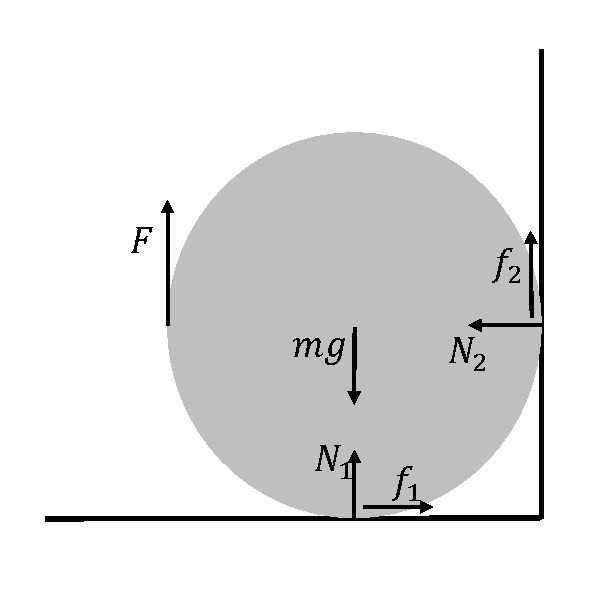
\includegraphics[width=\linewidth]{Fig1.pdf}
		\caption{\label{fig:fig1}}
	\end{subfigure}%
	\begin{subfigure}[t]{.3\linewidth}
		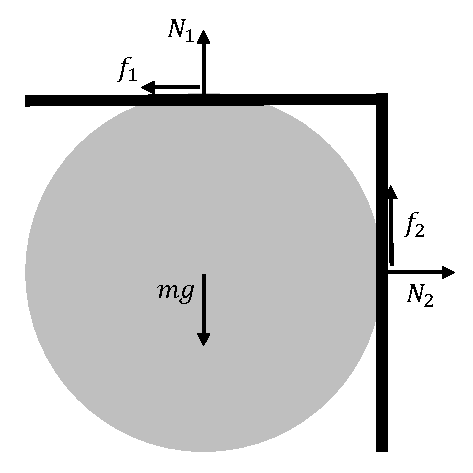
\includegraphics[width=\linewidth]{Fig2.pdf}
		\caption{\label{fig:fig2}}
	\end{subfigure}
	\caption{\subref{fig:fig1} 고급물리학 1차 과제 문제 5번 \subref{fig:fig2} 고급물리학 2차 과제 문제 11번}
\end{figure}
이 문서에서는 그림 \ref{fig:fig1}에 해당하는 문제를 풀이한다.
\begin{align}
& \text{토크평형} & F&=f_{1}+f_{2} \label{torque} \\
& \text{$x$방향 힘평형} & f_{1}&=N_{2} \label{x} \\
& \text{$y$방향 힘평형} & mg&=F+N_{1}+f_{2} \label{y} \\
& \text{마찰계수 고려} & f_{1} &\leq \mu N_{1} \label{f1} \\
& & f_{2} &\leq \mu N_{2} \label{f2}
\end{align}
식 \eqref{torque} - \eqref{f2}\를 $ f_{1} $, $ f_{2} $에 대해 정리하자.
\eqref{y} 에 \eqref{torque}\를 대입하면 식 \eqref{n1}\이 되고, \eqref{x}\를 다시 쓰면 \eqref{n2}\가 된다.
\begin{align}
N_{1} &= mg-f_{1}-2f_{2} \label{n1} \\
N_{2} &= f_{1} \label{n2}
\end{align}
식 \eqref{n1}, \eqref{n2}\를 조건 \eqref{f1}, \eqref{f2}에 대입하여 정리하면, 부등식 \eqref{inequality}\를 얻는다.
\begin{equation} \label{inequality}
\begin{cases}
(1/\mu+1)f_{1}+2f_{2} \leq mg \\
f_{2} \leq \mu f_{1} 
\end{cases}
\end{equation}
부등식 \eqref{inequality} 에 의거하여 영역을 그려보면 그림 \ref{0.4}와 같다. 부등식의 영역은 삼각형이다.

이제 우리가 할 일은 원통이 미끄러지지 않기 위한 힘 $F$의 최대값을 구하는 것이다. 직선 $ F=f_{1}+f_{2} $ 을 $ F=\infty $ 에서 시작하여 점점 줄여나가다가, 그러다가 직선이 삼각형 영역과 처음으로 만나는 순간이 $ F $가 최대인 순간이다.

\begin{figure}[t]
	\centering
	\begin{subfigure}[b]{0.3\linewidth}
		\centering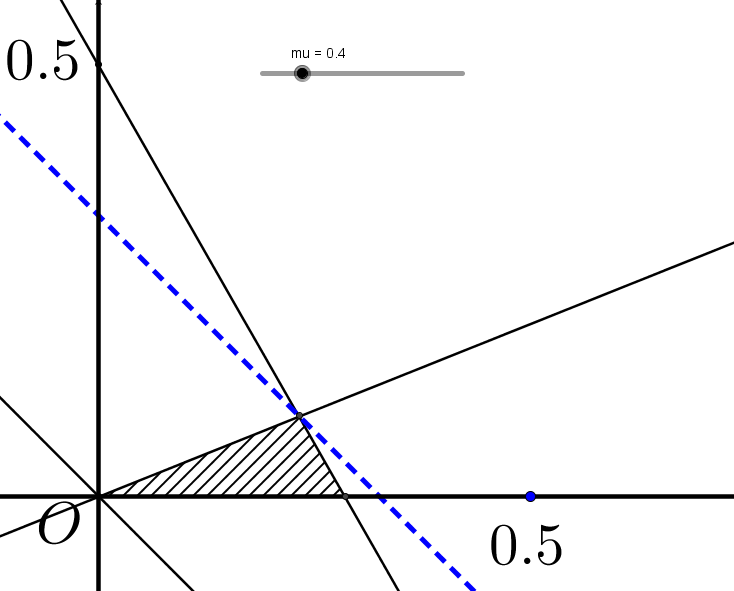
\includegraphics[width=\linewidth]{mu04_v3.png}
		\caption{\label{0.4}}
	\end{subfigure}
	~
	\begin{subfigure}[b]{0.3\linewidth}
		\centering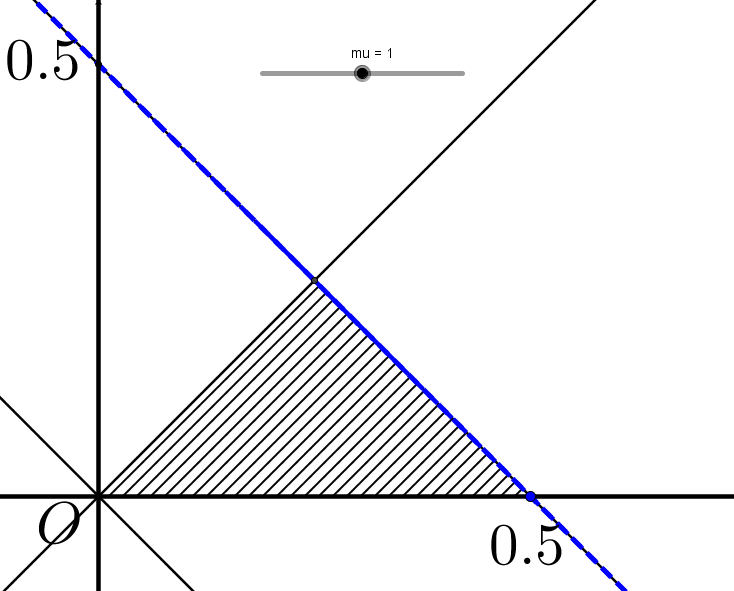
\includegraphics[width=\linewidth]{mu10_v3.png}
		\caption{\label{1.0}}
	\end{subfigure}
	~
	\begin{subfigure}[b]{0.3\linewidth}
		\centering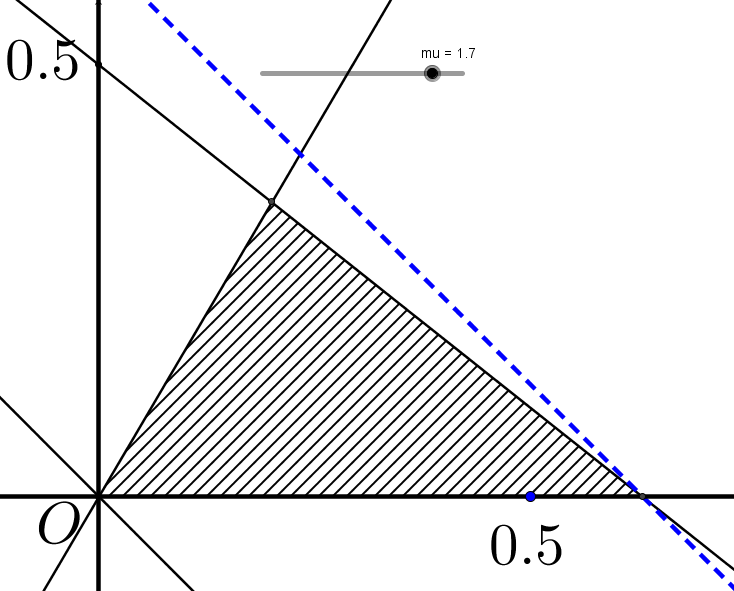
\includegraphics[width=\linewidth]{mu17_v3.png}
		\caption{\label{1.4}}
	\end{subfigure}
	\caption{$\mu$가 \subref{0.4} : $0.4$, \subref{1.0} : $1.0$, \subref{1.4} : $1.7$ 일 때의 그래프. $x$축은 $f_{1}$, $y$축은 $f_{2}$ 이며, 단위는 $mg$ 이다.}
\end{figure}

그림 \ref{0.4}를 보면, $ f_{1}=\mu N_{1} $, $ f_{2}=\mu N_{2} $ 인 경우가 $F$가 최대인 때이다. 이것이 보통 사용되는 풀이다. 하지만, 만약 $\mu$ 가 1보다 크다면 어떻게 될까? \footnote{보통의 경우 정지마찰계수 $\mu$ 는 1보다 작지만, 검색을 조금만 해보면 그렇지 않은 경우가 상당히 있다는 것을 알 수 있다.} 그림 \ref{1.0} 와 \ref{1.4}\를 보라. 무언가가 이상함을 눈치챘는가? $\mu > 1$ 일때는 $F$가 최대인 때가 $ f_{1}=\mu N_{1} $, $ f_{2}=\mu N_{2} $ 일 때가 아닌 $f_{2}=0$ 일 때이다!

정확한 답은 \eqref{answer}와 같이 $\mu$ 의 값에 따라 나뉨을 알 수 있다.

\begin{equation} \label{answer}
F_{max} = 
\begin{cases}
\frac{\mu^{2}+\mu}{2\mu^{2}+\mu+1} mg & (\mu < 1)\\ 
\frac{\mu}{\mu+1} mg & (\mu > 1) 
\end{cases}
\end{equation}
참고로 $\mu$ 의 값에 따른 $F_{max}$ 의 그래프는 그림 \ref{answergraph} 와 같다.

저자 주 : 그림 \ref{fig:fig2} 에 해당하는 문제도 이와 같이 풀 수 있다. $N_{1}$, $N_{2}$에 대해 정리하면 편하며, 기울기가 $\mu$, $-1/\mu$인 두 직선(직교한다!)에 의한 부등식의 영역이 나타난다. 기하적인 방법을 이용하여, 해결할 수 있다. 답 : $\mu < \tan{22.5^{\circ}} = \sqrt{2}-1$ ($ N_{2}-N_{1} $ 그래프에서 두 직선의 교점은 항상 $ (mg,0) $이 중심이고 반지름이 $ mg $인 원 위에 있음을 이용하면 좋다.)
\begin{figure}[b]
	\centering
	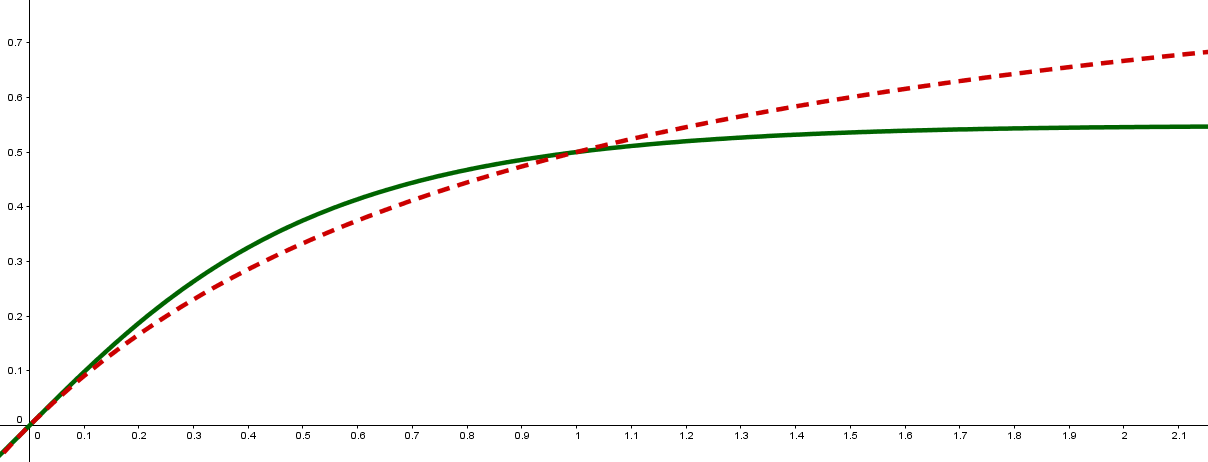
\includegraphics[width=.5\linewidth]{answer_v4.png}
	\caption{$F_{max}(\mu)$. $x$축은 $\mu$, $y$축은 $F_{max}$(단위 : $mg$). 실선이 $\mu<1$에, 점선이 $\mu>1$에 해당된다.}
	\label{answergraph}
\end{figure}
\end{document}
